\documentclass{scalatekids-article}
\usepackage[official]{eurosym}
\begin{document}
\lfoot{Developer Manual 1.0.0}
\newgeometry{top=3.5cm}
\begin{titlepage}
  \begin{center}
    \begin{center}
      
\includegraphics[width=10cm]{sklogo.png}
    \end{center}
    \vspace{1cm}
    \begin{Huge}
      \begin{center}
        \textbf{Developer Manual}
      \end{center}
    \end{Huge}
    \vspace{11pt}
    \bgroup
    \def\arraystretch{1.3}
    \begin{tabular}{r|l}
      \multicolumn{2}{c}{\textbf{Informazioni sul documento}} \\
      \hline
      \setbox0=\hbox{0.0.1\unskip}\ifdim\wd0=0pt
      \\
      \else
      \textbf{Versione} & 1.0.0\\
      \fi
      \textbf{Editing} & \multiLineCell[t]{\\}\\
      \textbf{Verification} & \multiLineCell[t]{\\}\\
      \textbf{Approvation} & \multiLineCell[t]{}\\
      \textbf{Use} & External\\
      \textbf{Distribution List} & \multiLineCell[t]{ScalateKids\\Prof. Tullio Vardanega\\Prof. Riccardo Cardin}\\
    \end{tabular}
    \egroup
    \vspace{22pt}
  \end{center}
\end{titlepage}
\restoregeometry
\clearpage
\pagenumbering{Roman}
\setcounter{page}{1}
\begin{flushleft}
  \vspace{0cm}
  {\large\bfseries History log}
\end{flushleft}
\vspace{0cm}
\begin{center}
  \begin{tabular}{| l | l | l | l | p{5cm} |}
    \hline
    Version & Author & Role & Date & Description \\
    \hline
    0.1.1 & Andrea Giacomo Baldan & Programmer & 2016-05.12 & Added section 2.3\\
    \hline
    0.1.0 &  &  & 2016-05-10 & Verified section 2: Actorbase Usage and all relative subsections\\
    \hline
    0.0.2 & Andrea Giacomo Baldan & Programmer & 2016-05-10 & Added section 2: Actorbase Usage and all relative subsections\\
    \hline
    0.0.1 & Andrea Giacomo Baldan & Programmer & 2016-05-10 & Created document structure\\
    \hline
  \end{tabular}
\end{center}
\tableofcontents
\newpage
\pagenumbering{arabic}
\section{Summary}
\subsection{Document purpose}
This document aim to describe the procedures and methods to use in order to take advantage of \gloss{Actorbase}.

\subsection{References}

\subsubsection{Normative} % TODO check, translated with wordreference

\subsubsection{Informational} % TODO check, translated with wordreference

% TODO parte server: installazione, configurazione, accensione, spegnimento

% TODO mettere una sezione in cui si spiega cosa è una collection, un item, tutto quel che bisogna descrivere

% TODO bisogna spiegare come devnoon essere formati i file pel l'import

%%%%%%%%%%%%%%%%%%%%%%%%%%%%%%%%%%%%%%%%%%%%%%%%%%%%%%%%%%%%%%%%%%%%
%%% INSTALLATION PART                    %%%
%%%%%%%%%%%%%%%%%%%%%%%%%%%%%%%%%%%%%%%%%%%%%%%%%%%%%%%%%%%%%%%%%%%%


%%%%%%%%%%%%%%%%%%%%%%%%%%%%%%%%%%%%%%%%%%%%%%%%%%%%%%%%%%%%%%%%%%%%
%%%%%%%%%%%% MACHETE                   %%%%%%%%%%%%
%%%%%%%%%%%%%%%%%%%%%%%%%%%%%%%%%%%%%%%%%%%%%%%%%%%%%%%%%%%%%%%%%%%%


%%%%%%%%%%%%%%%%%%%%%%%%%%%%%%%%%%%%%%%%%%%%%%%%%%%%%%%%%%%%%%%%%%%%
%%% DRIVER PART                          %%%
%%%%%%%%%%%%%%%%%%%%%%%%%%%%%%%%%%%%%%%%%%%%%%%%%%%%%%%%%%%%%%%%%%%%

\section{Actorbase usage}

\subsection{Installation}
% TODO

\subsection{Distribution: Cluster configuration}
% TODO

\subsection{ActorbaseDriver: Using Actorbase from inside a Scala source}

Actorbase is essentially an actor system built upon a server component that
exposes some API forming a RESTful web service. To facilitate the use from
inside a Scala source, it has been developed a driver in order to allow the
usage of all features that Actorbase provides.\\

\subsubsection{Quick Start: a generic example}

The most common operations include:
\begin{itemize}
\item Authentication;
\item Profile management operations;
\item Collections operations;
\item Administrative operations.
\end{itemize}

\begin{figure}[H]
  \begin{center}
    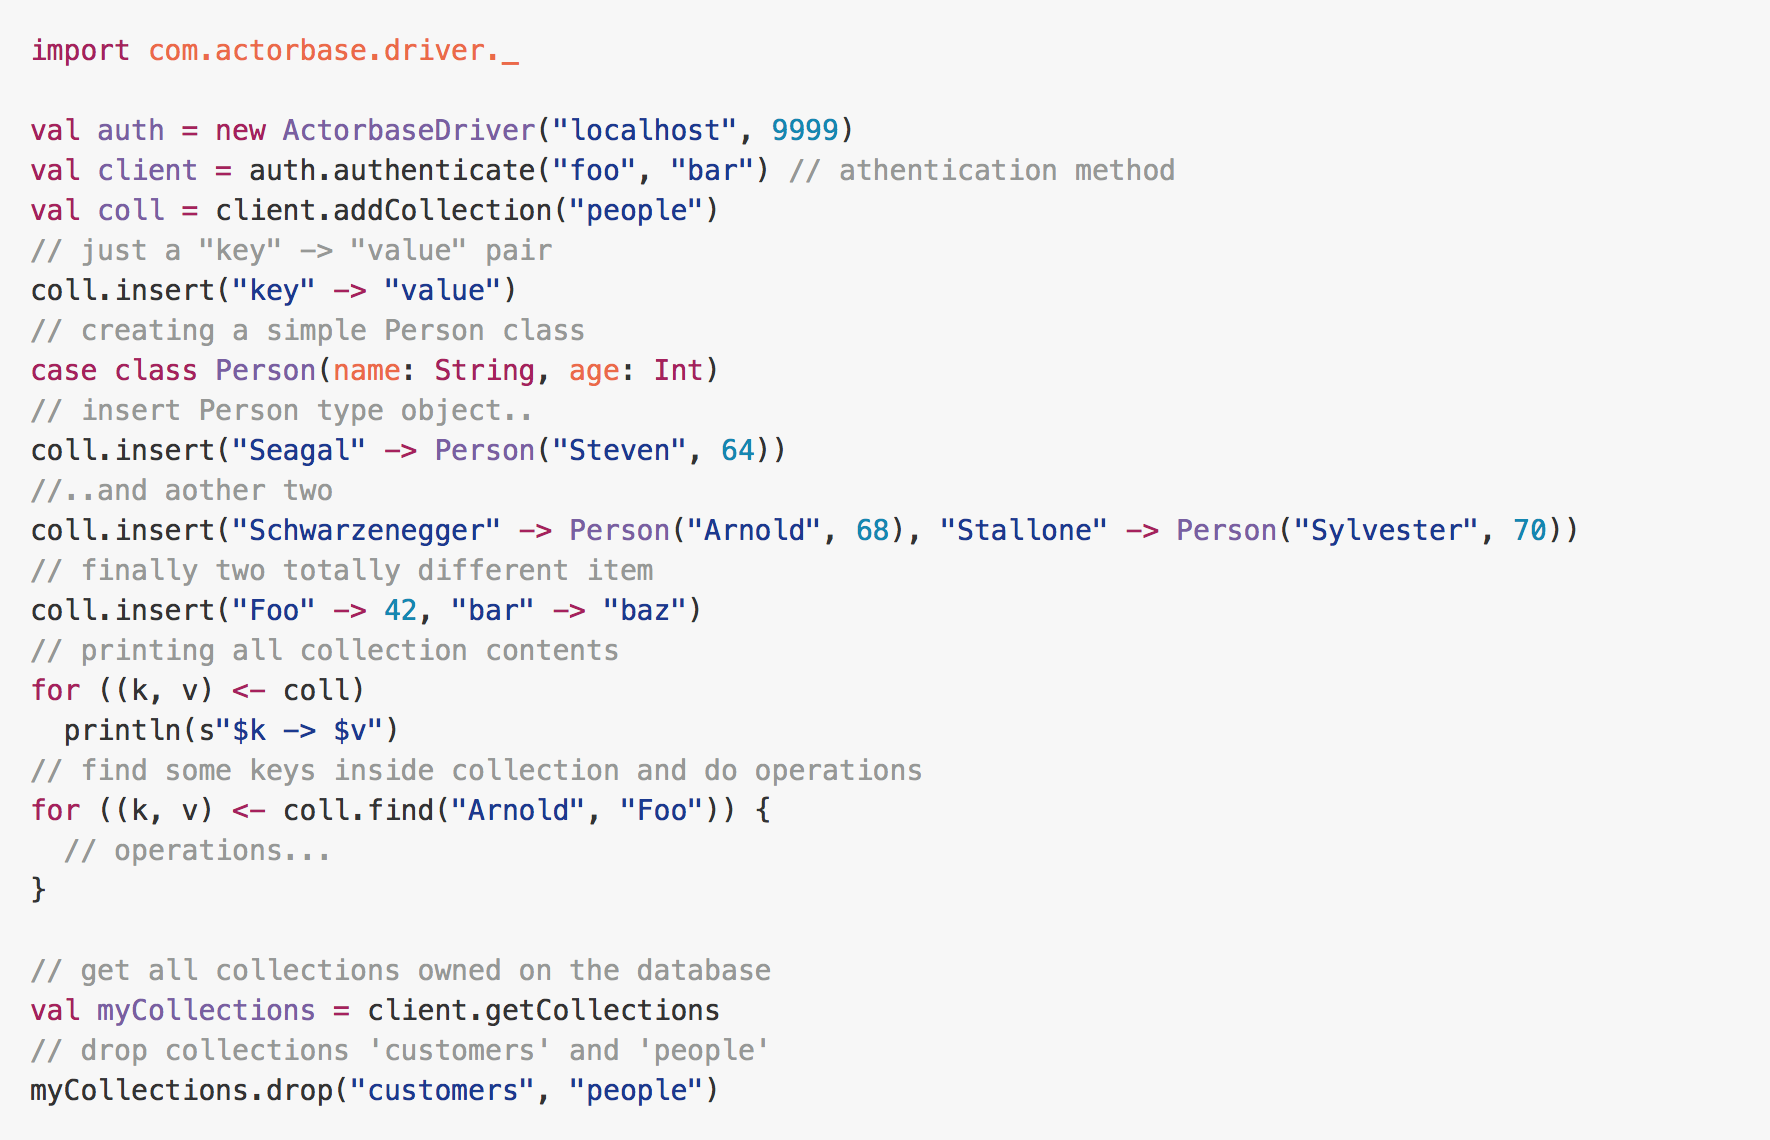
\includegraphics[width=0.9\textwidth,keepaspectratio]{RQ/DevManual/Driver-Common.png}
    \caption{Driver usage: Generic example}
  \end{center}
\end{figure}

These are some of the most common operations that the driver allows to do,
there's not too much boilerplate\footnote{A section of code that have to be
  included in many places with little to no alteration.} code, and it's possible
to make operations directly on objects representing \textbf{Actorbase}
collections\footnote{A data-structure constituted by a list of key-value items\label{coll}}
in a purely OOP (Object Oriented Programming) fashion.\\ As explained in
the snippet\footnote{A programming term for a small region of reusable code.}
image, these objects also retain some of the common functional constructs (e.g.
foreach), so it's possible to apply custom functions to every item of the
collection.

\subsection{More in depth: common operations}

\paragraph{Authentication}

Althrough in the future perhaps there could be the possibility to make some
operations as an anonymous user, at the current state the only possible action
that a non-logged-in user can do with ActorbaseDriver is the authentication.
This method send a login request to the server-side of the system and, according
to the response, it will return an \verb=ActorbaseService=\footnote{Main class,
  contains all collection management methods\label{ActorbaseServices}} or an
\verb=ActorbaseAdminServices=\footnote{Defined trait, contains some
  administrative functionality as dependancy added to
  ActorbaseServices\label{AdminService}}. These two objects give the methods to
actually make all operations on the database, the main difference is that
\verb=ActorbaseAdminServices=\textsuperscript{\ref{AdminServices}} allows to do
some high-level administrative operations on users and
collections\textsuperscript{\ref{coll}} of the system. Authentication method
could raise \textbf{WrongCredentialExc} exception, in case of worng credentials
sent to the server.

\paragraph{Profile management}

\textit{ActorbaseDriver} provides a method to modify the current password,
associated to an user profile.
e.g.:
% \begin{figure}[H]
%   \begin{center}
%     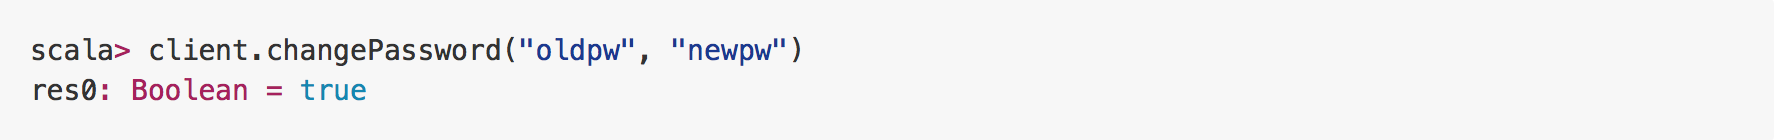
\includegraphics[width=0.9\textwidth,keepaspectratio]{RQ/DevManual/Driver-UserManagement.png}
%     \caption{Driver usage: insertion methods}
%   \end{center}
% \end{figure}
This method could raise:
\begin{itemize}
\item \textbf{WrongPasswordExc} In case of a wrong current password;
\item \textbf{WrongNewPasswordExc} In case of a new password that don't matches \textbf{Actorbase} password rules.
\end{itemize}

\subparagraph{Credential rules}
% TODO: Complete
Password must be at least 8 characters length.

\paragraph{Collections operations}

As previously explained, operations on the collections\textsuperscript{\ref{coll}} can be done in a purely
OOP way, this mean that all methods that return an \verb=ActorbaseCollection=,
gives the possibility to call all collection-management methods:
\begin{itemize}
\item \verb=listCollection=, lists all collections\textsuperscript{\ref{coll}}
  contained in the database, these are collections\textsuperscript{\ref{coll}}
  owned by the profile of the requester, including contributions ones.
\item \verb=addCollection= method:\\ Create a new collection\textsuperscript{\ref{coll}} into \textbf{Actorbase}, accepting a \verb=String=
  representing the name of the new collection\textsuperscript{\ref{coll}};
  e.g.:
  % \begin{figure}[H]
  %   \begin{center}
  %     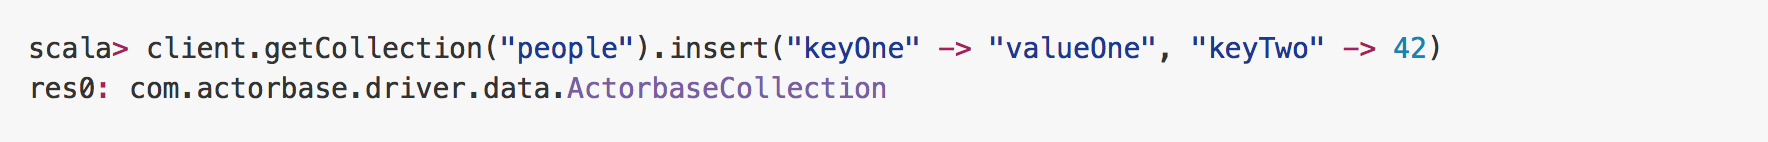
\includegraphics[width=0.9\textwidth,keepaspectratio]{RQ/DevManual/Driver-Insert.png}
  %     \caption{Driver usage: insertion methods}
  %   \end{center}
  % \end{figure}
  Add collection\textsuperscript{\ref{coll}} method could raise:
  \begin{itemize}
  \item \textbf{CollectionAlreadyExistsExc:} In case of duplicate collection\textsuperscript{\ref{coll}} name into \textbf{Actorbase};
  \item \textbf{UndefinedCollectionExc:} In case of addition of a new collection\textsuperscript{\ref{coll}} with an empty name.
  \end{itemize}
\item \verb=insert= methods:\\ These methods come in two variants, first one accepting
  a vararg\footnote{A sequence of arguments} of key-value tuple, the second
  accepting an
  \verb=ActorbaseObject=\footnote{An object representing a key-value pair inside Actorbase} instance;
  e.g.:
  % \begin{figure}[H]
  %   \begin{center}
  %     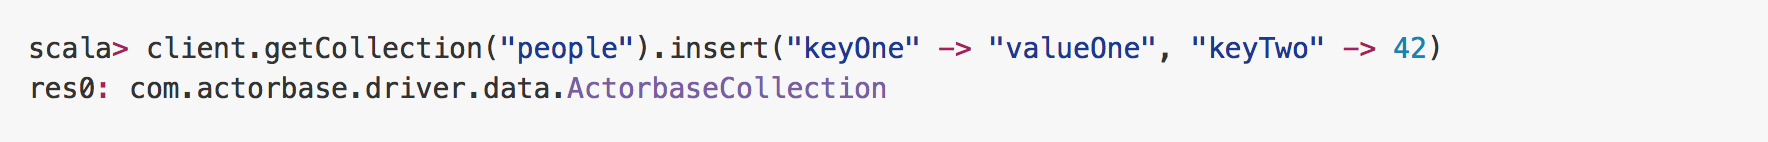
\includegraphics[width=0.9\textwidth,keepaspectratio]{RQ/DevManual/Driver-Insert.png}
  %     \caption{Driver usage: insertion methods}
  %   \end{center}
  % \end{figure}
  Insert methods could raise:
  \begin{itemize}
  \item \textbf{DuplicateKeyExc:} In case of a key already present inside the collection\textsuperscript{\ref{coll}}.
  \end{itemize}
\item \verb=remove= methods:\\ There're two variants of this method too, the usage is
  analogous to insert, e.g.:
  % \begin{figure}[H]
  %   \begin{center}
  %     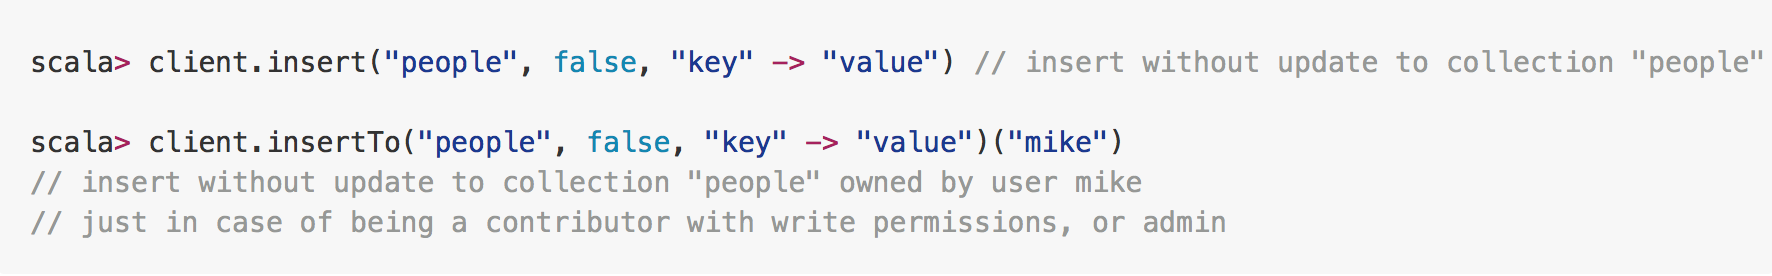
\includegraphics[width=0.9\textwidth,keepaspectratio]{RQ/DevManual/Driver-Insert2.png}
  %     \caption{Driver usage: remove methods}
  %   \end{center}
  % \end{figure}
\item \verb=find= method:\\ This method accept one or more \verb=String= representing
  keys to be retrieved from the collection\textsuperscript{\ref{coll}}, again the usage is similar to insert and
  remove methods, e.g.:
  % \begin{figure}[H]
  %   \begin{center}
  %     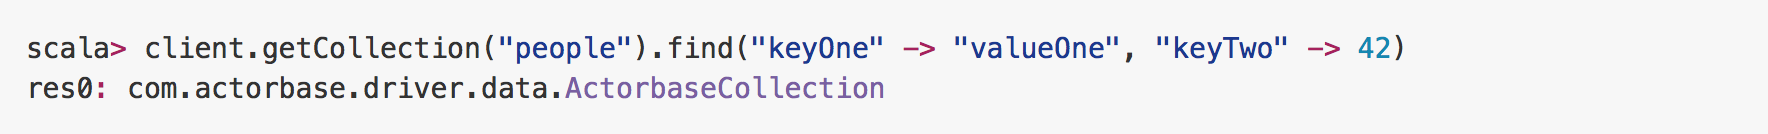
\includegraphics[width=0.9\textwidth,keepaspectratio]{RQ/DevManual/Driver-Find.png}
  %     \caption{Driver usage: find method}
  %   \end{center}
  % \end{figure}
\item \verb=findOne= method:\\ This method accept one \verb=ActorbaseObject= representing
  a key-value pair to be retrieved from the collection\textsuperscript{\ref{coll}}, again the usage is similar to insert and
  remove methods, e.g.:
  % \begin{figure}[H]
  %   \begin{center}
  %     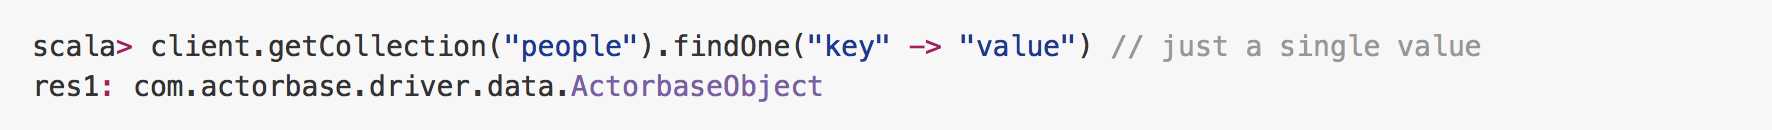
\includegraphics[width=0.9\textwidth,keepaspectratio]{RQ/DevManual/Driver-FindOne.png}
  %     \caption{Driver usage: findOne method}
  %   \end{center}
  % \end{figure}
\item \verb=drop= methods:\\ Again this method have multiple variants, there's the
  \verb=dropCollections= that can be used to wipe out all the database, e.g.:
  % \begin{figure}[H]
  %   \begin{center}
  %     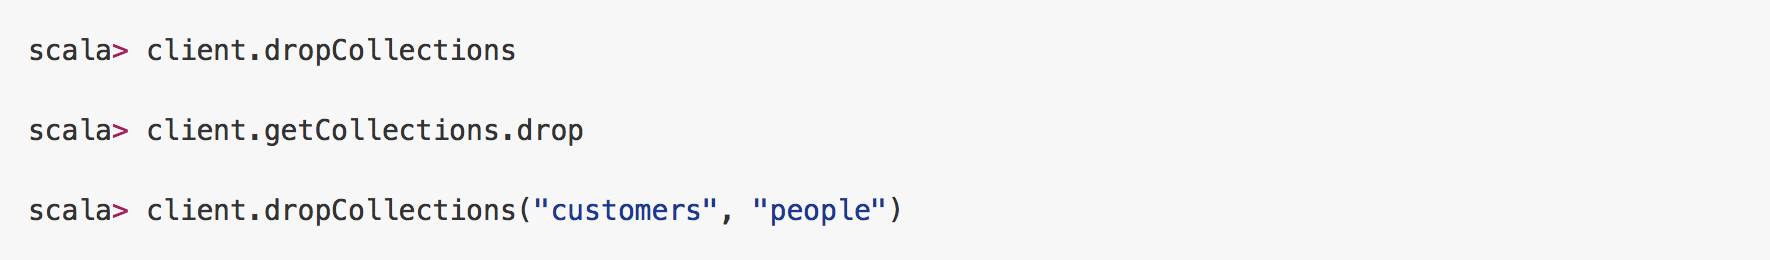
\includegraphics[width=0.9\textwidth,keepaspectratio]{RQ/DevManual/Driver-DropCollections.png}
  %     \caption{Driver usage: dropCollections method}
  %   \end{center}
  % \end{figure}
  the \verb=drop= inside an \verb=ActorbaseCollection= object:
  % \begin{figure}[H]
  %   \begin{center}
  %     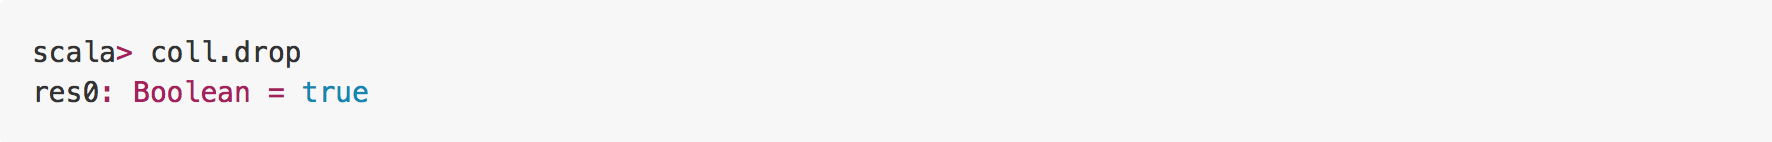
\includegraphics[width=0.9\textwidth,keepaspectratio]{RQ/DevManual/Driver-Drop.png}
  %     \caption{Driver usage: drop method}
  %   \end{center}
  % \end{figure}
  and finally \verb=drop= inside an \verb=ActorbaseCollectionMap=, it takes a
  vararg of \verb=String= representing a sequence of collections\textsuperscript{\ref{coll}} to be removed
  e.g.:
  % \begin{figure}[H]
  %   \begin{center}
  %     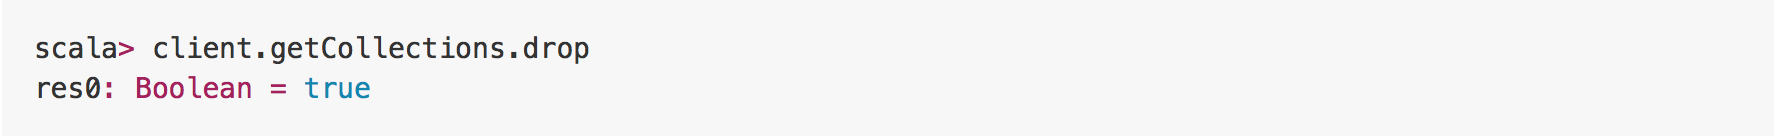
\includegraphics[width=0.9\textwidth,keepaspectratio]{RQ/DevManual/Driver-Drop2.png}
  %     \caption{Driver usage: drop method}
  %   \end{center}
  % \end{figure}
\item printing collections\textsuperscript{\ref{coll}}:\\All object returned by \verb=ActorbaseDriver=
  have an override\footnote{Specific implementation of a method in a subclass that
    is already provided by one of its superclasses} to the method \verb=toString=
  that return a pretty formatted JSON(JavaScript Object Notation) \verb=String=, e.g.:
  % \begin{figure}[H]
  %   \begin{center}
  %     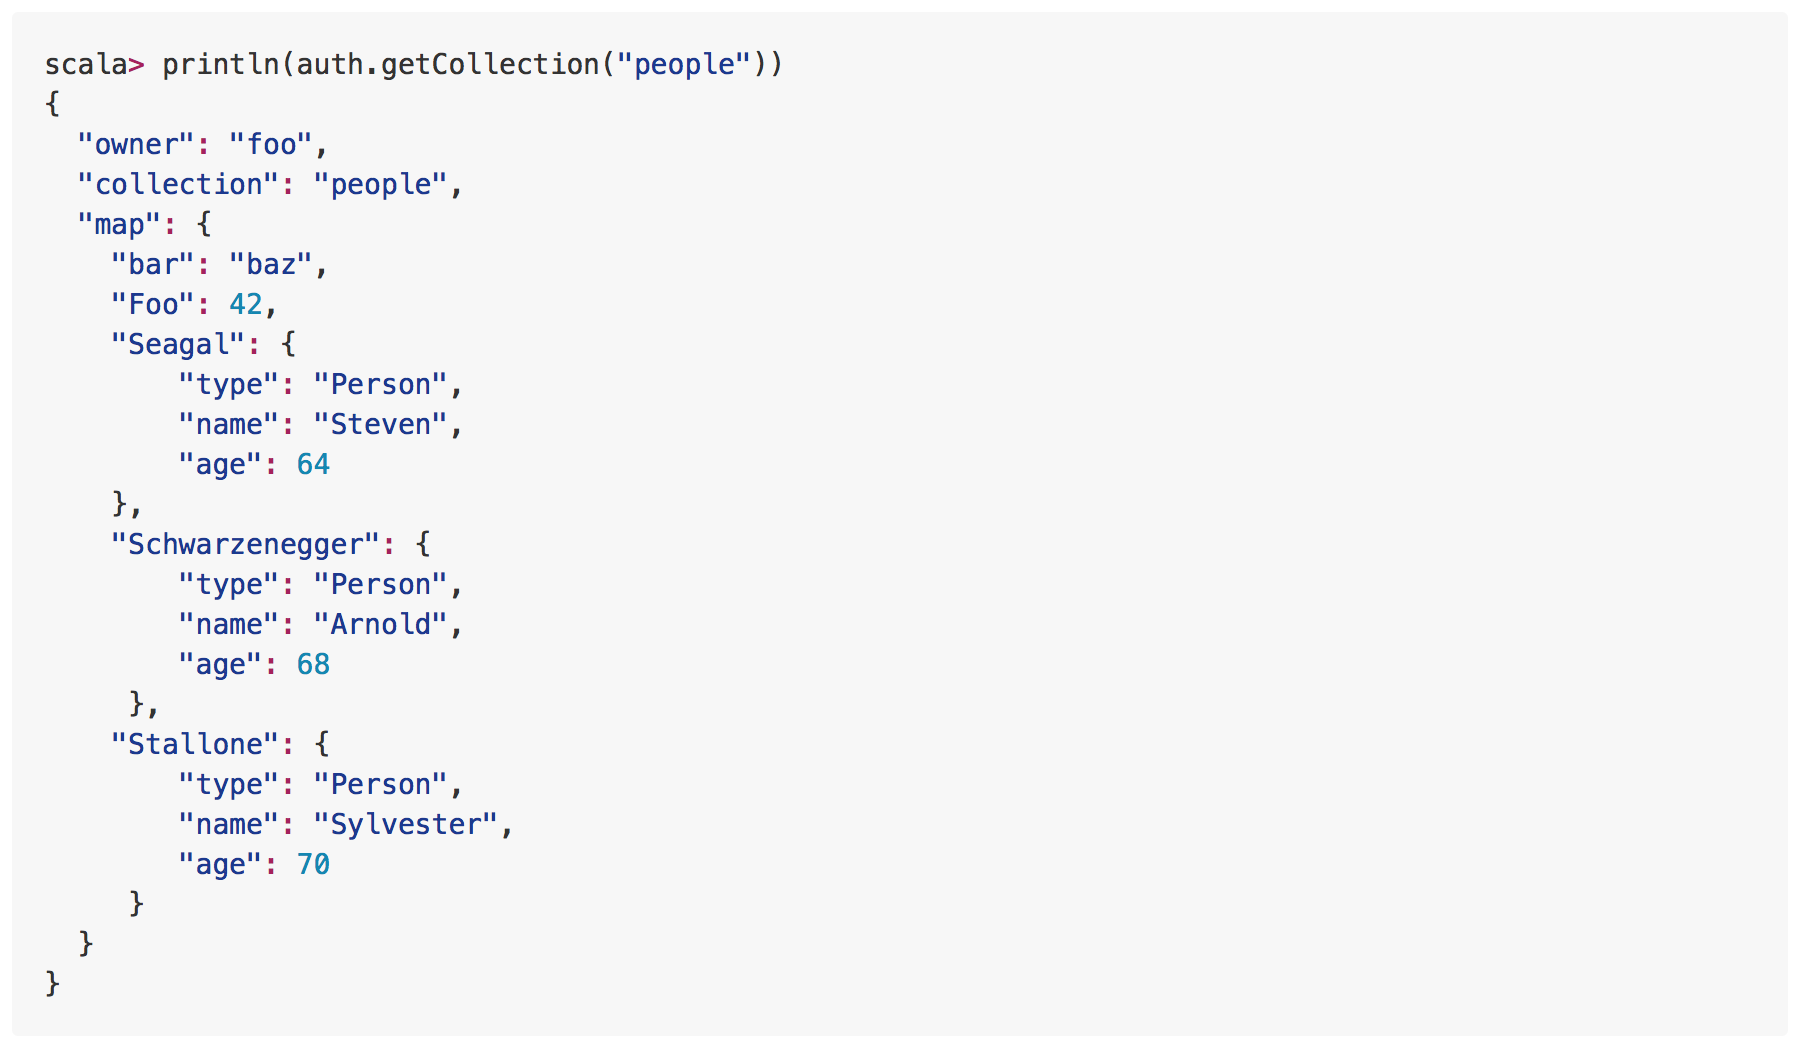
\includegraphics[width=0.9\textwidth,keepaspectratio]{RQ/DevManual/Driver-Printing.png}
  %     \caption{Driver usage: drop method}
  %   \end{center}
  % \end{figure}
\item \verb=count= elements inside a collection\textsuperscript{\ref{coll}} e.g.
  % \begin{figure}[H]
  %   \begin{center}
  %     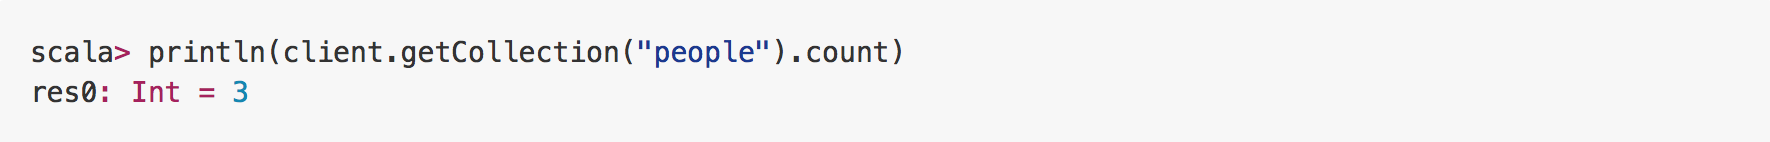
\includegraphics[width=0.9\textwidth,keepaspectratio]{RQ/DevManual/Driver-Counting.png}
  %     \caption{Driver usage: drop method}

  %   \end{center}
  % \end{figure}
\item \verb=importFromFile=, method that allow to import a (possibly) large number of collections\textsuperscript{\ref{coll}}
  directly into \textbf{Actorbase}
  % \begin{figure}[H]
  %   \begin{center}
  %     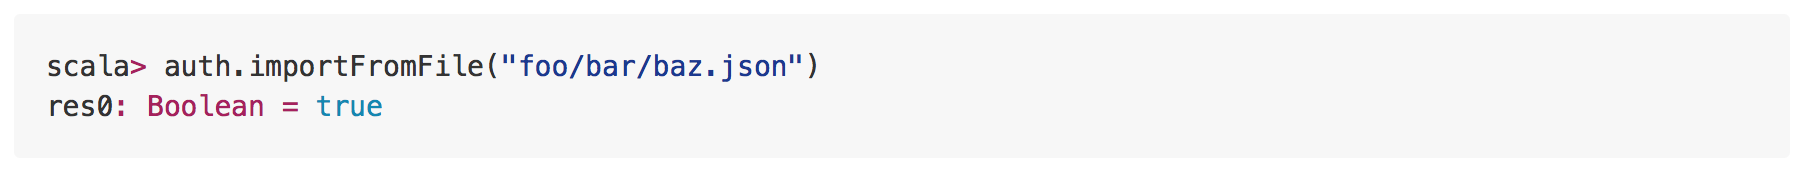
\includegraphics[width=0.9\textwidth,keepaspectratio]{RQ/DevManual/Driver-Import.png}
  %     \caption{Driver usage: import from file method}

  %   \end{center}
  % \end{figure}
  This method could raise:
  \begin{itemize}
  \item \textbf{UndefinedFileExc:} in case of file not found at the given path in the filesystem;
  \item \textbf{MalformedFileExc:} in case of a file not in JSON format or not valid JSON.
  \end{itemize}

\item \verb=exportToFile=, method that allow to export one or more collections\textsuperscript{\ref{col}} to a specified path on the filesystem
  % \begin{figure}[H]
  %   \begin{center}
  %     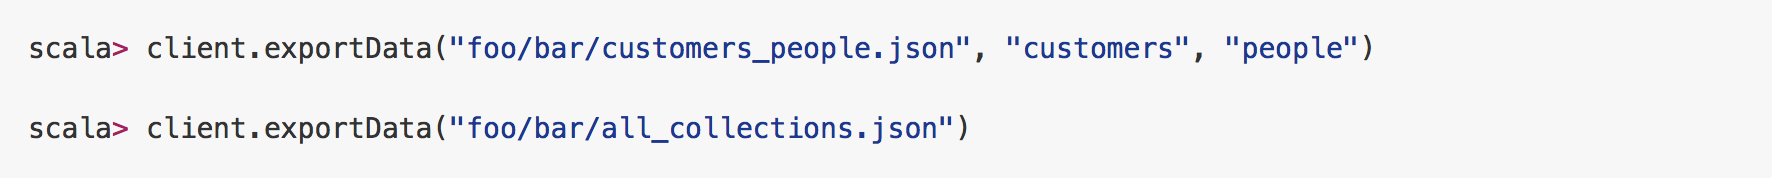
\includegraphics[width=0.9\textwidth,keepaspectratio]{RQ/DevManual/Driver-Export.png}
  %     \caption{Driver usage: export to file method}

  %   \end{center}
  % \end{figure}
\end{itemize}

\subparagraph{Contributor management}

Each user in \textbf{Actorbase} have the possibility to add and remove contributors
to his collections\textsuperscript{\ref{coll}}, a user can be added with two level of
permission:
\begin{itemize}
\item read, means that a user can only make read operations on the collection\textsuperscript{\ref{coll}} without modifying it;
\item read-write, means that a user can make read and write operations on the collection\textsuperscript{\ref{coll}}.
\end{itemize}
e.g.:
% \begin{figure}[H]
%   \begin{center}
%     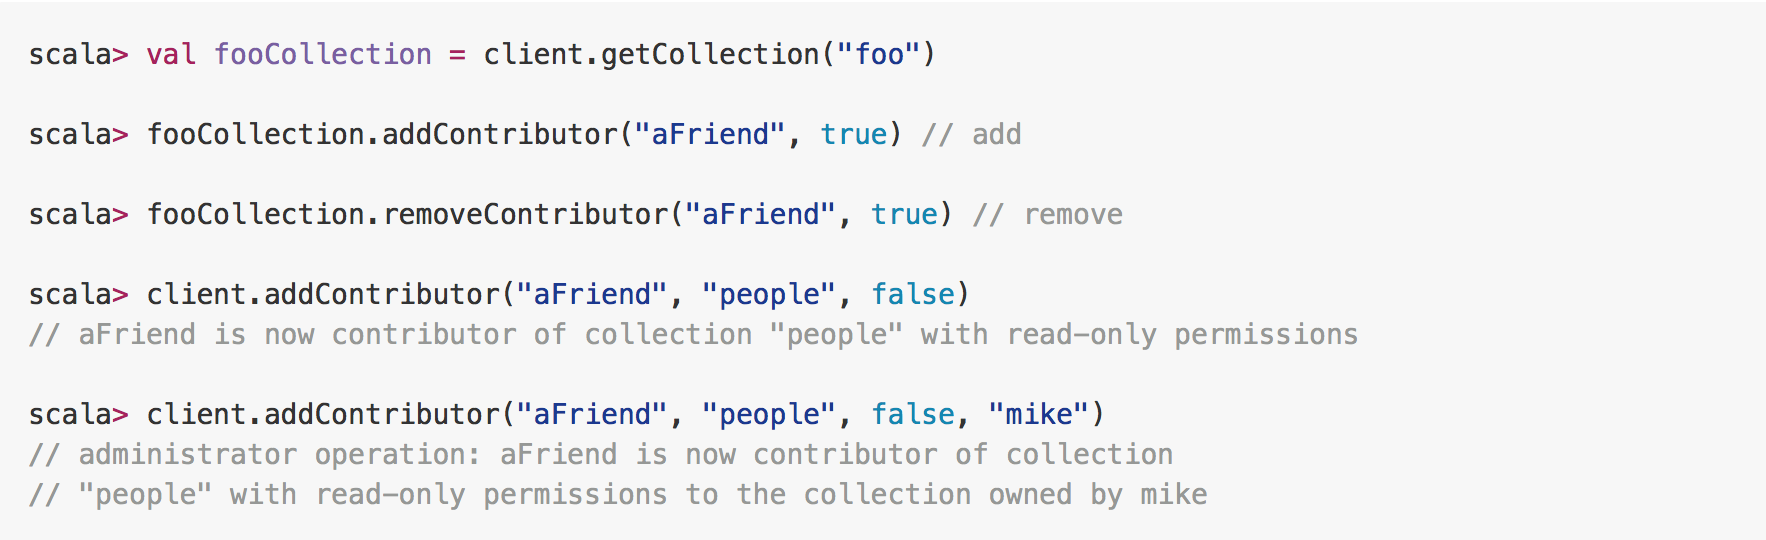
\includegraphics[width=0.9\textwidth,keepaspectratio]{RQ/DevManual/Driver-Contributor.png}
%     \caption{Driver usage: drop method}
%   \end{center}
% \end{figure}

\paragraph{Administrative operations}

Actorbase expect two kind of users, common an administrator. The last one have
some privileges over the others, such as a wider range of collections\textsuperscript{\ref{coll}} (all
database) with read-write permissions, and capabilities of adding and removing
users to and from the system, and finally resetting the password of given users.
% \begin{figure}[H]
%   \begin{center}
%     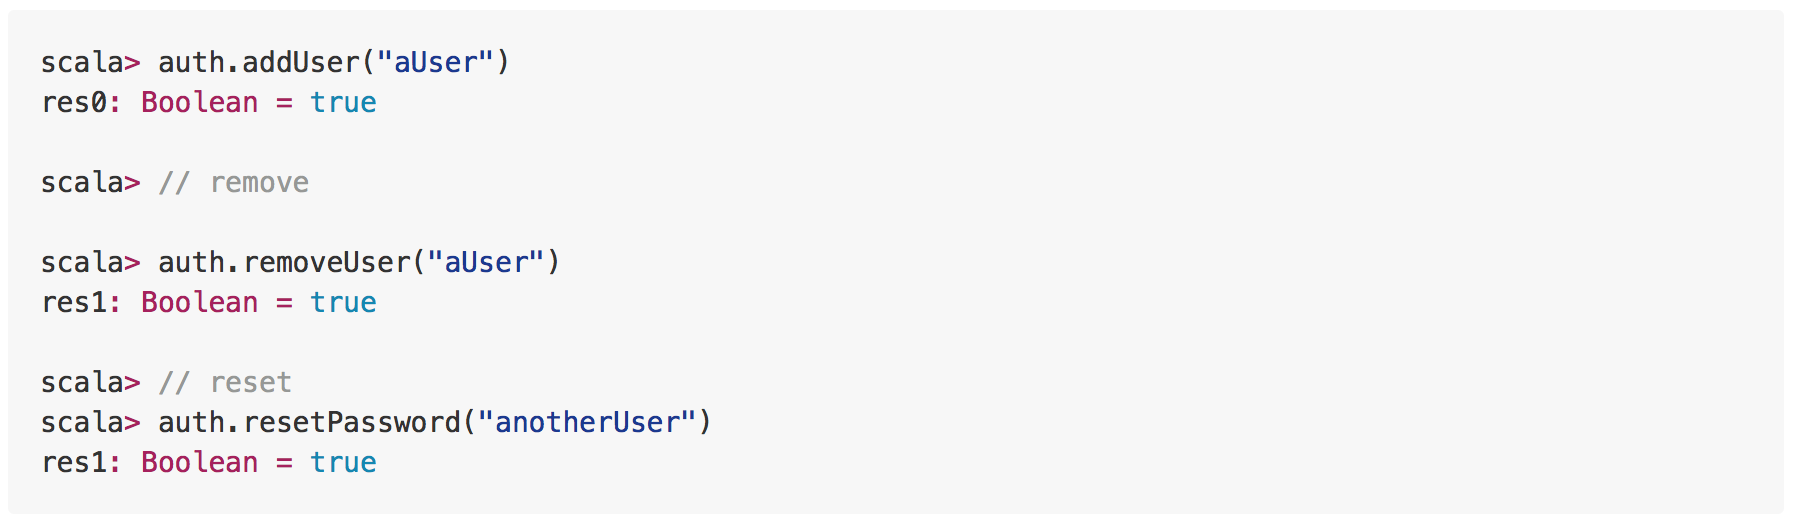
\includegraphics[width=0.9\textwidth,keepaspectratio]{RQ/DevManual/Driver-Administrative.png}
%     \caption{Driver usage: drop method}
%   \end{center}
% \end{figure}
Administrative operations could raise some exceptions:
\begin{itemize}
\item \textbf{UndefinedUsernameExc:} In case of addition of a new user with an empty username;
\end{itemize}
\paragraph{Error management}

There is one error that is shared by every method and that is in case of a
connection error, which can be caused by not receiving a response from the
server in a predetermined time, the driver will launch a timeout connection
exception. There are some errors that are specific to some methods, these will
be explained in the section dedicated to the methods that cause them.

% TODO: tutte le librerie utilizzate per la serializzazione

\end{document}